% Created 2016-09-01 Qui 09:40
\documentclass[11pt]{article}
\usepackage[utf8]{inputenc}
\usepackage[T1]{fontenc}
\usepackage{fixltx2e}
\usepackage{graphicx}
\usepackage{longtable}
\usepackage{float}
\usepackage{wrapfig}
\usepackage{rotating}
\usepackage[normalem]{ulem}
\usepackage{amsmath}
\usepackage{textcomp}
\usepackage{marvosym}
\usepackage{wasysym}
\usepackage{amssymb}
\usepackage{hyperref}
\tolerance=1000
\author{Cecília Carneiro e Silva}
\date{}
\title{TCC}
\hypersetup{
  pdfkeywords={},
  pdfsubject={},
  pdfcreator={Emacs 24.5.1 (Org mode 8.2.10)}}
\begin{document}

\maketitle
\tableofcontents


\section{{\bfseries\sffamily TODO} PICOBIT - pdf}
\label{sec-1}

Terminar de ler o artigo oficial do picobit.

\subsection{{\bfseries\sffamily TODO} Foto folha}
\label{sec-1-1}

Tirar foto da folha.

\begin{itemize}
\item SIXPIC C compiler é somente para PIC18.
\item Nesse caso vamos usar o cross-compiler: arm-none-eabi-gcc.
\end{itemize}

\subsection{{\bfseries\sffamily TODO} Comentarios}
\label{sec-1-2}

\begin{itemize}
\item Por causa do ambiente com tamanho de codigo limitado, todo projeto foi voltado a gerar bytecode compact code.
\item O bytecode resultante da scheme compiler é menor q o machine code, ou seja, o tamanho da entrada da VM é menor q a saída.
\item Como o projeto tem total controle, virtual machine e C compiler, podemos adaptar um ao outro.
\item A maquina virtual é escrita em C, tornando fácil a portabilidade entre hardwares, esse trabalho: STM32F1 e STM32F4.
\end{itemize}

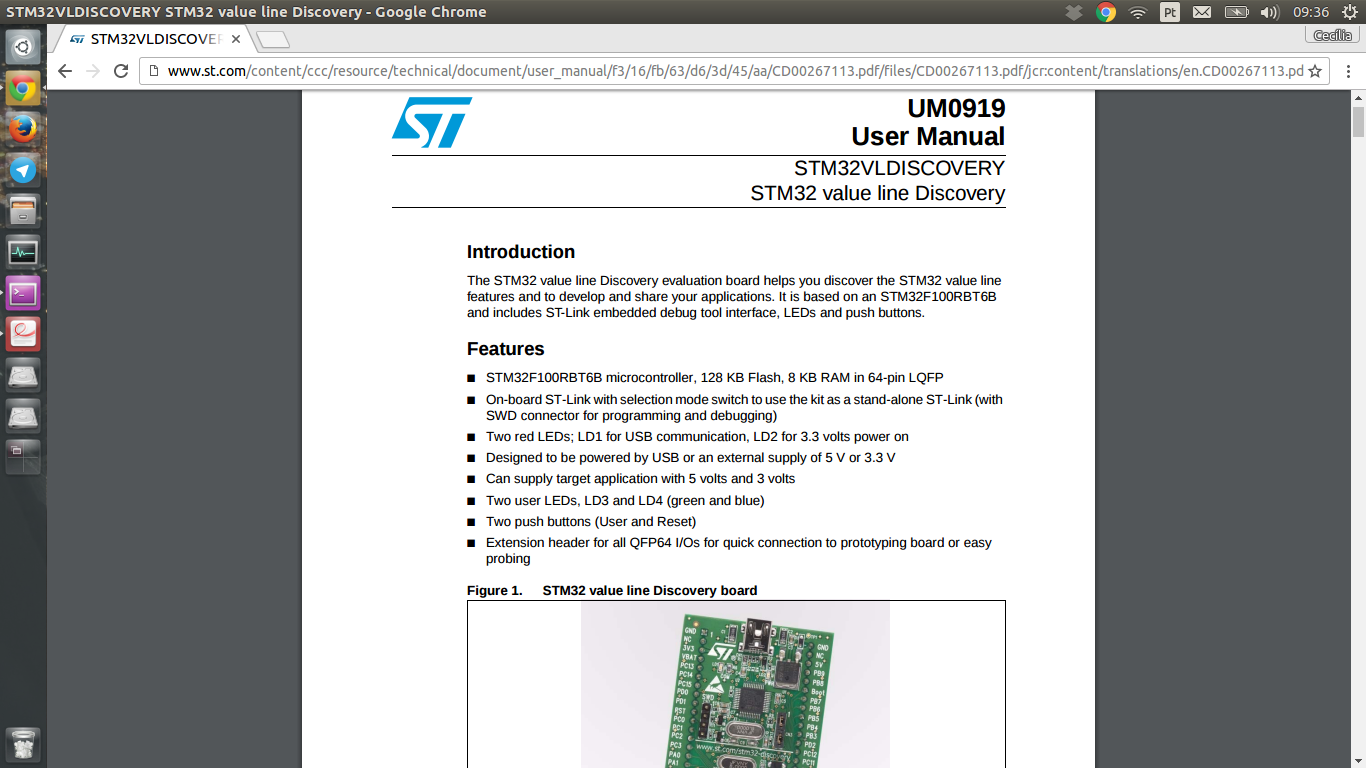
\includegraphics[width=.9\linewidth]{stm32f1.png}

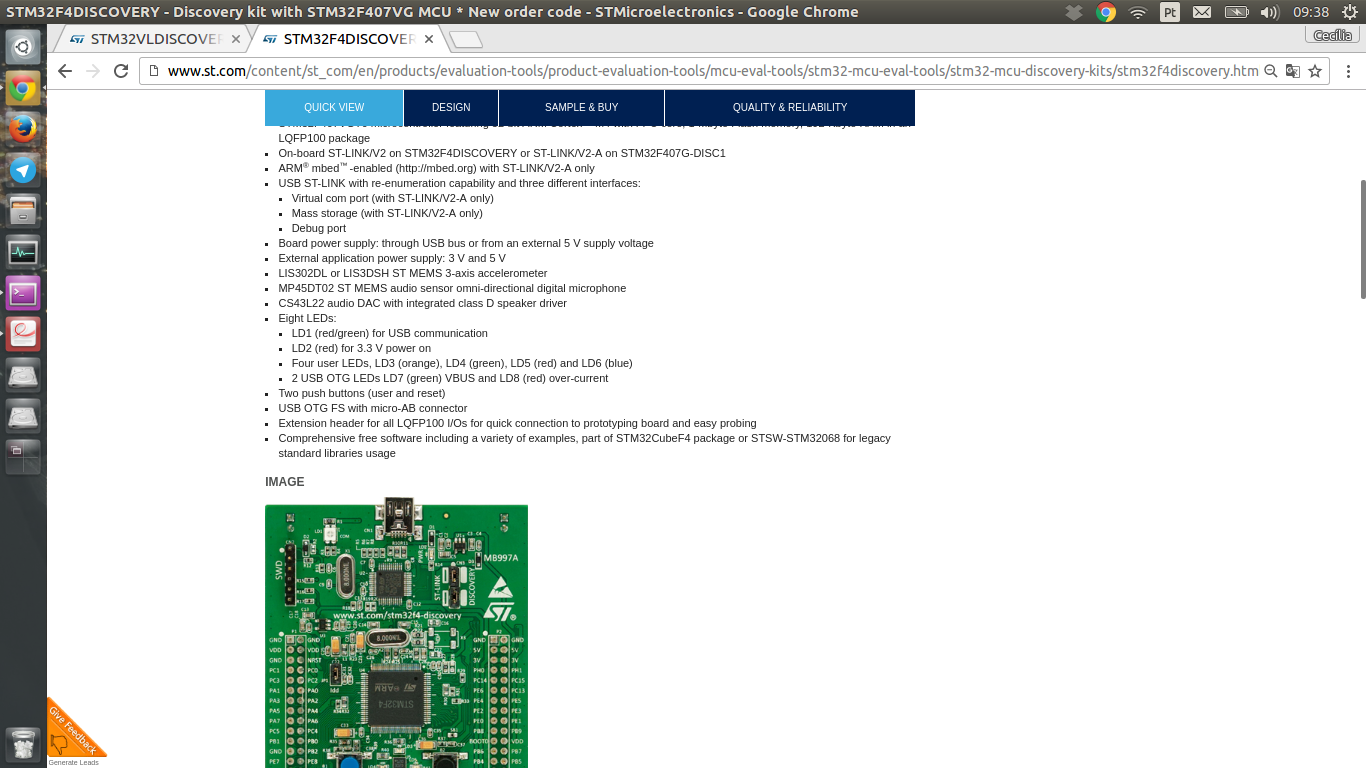
\includegraphics[width=.9\linewidth]{stm32f4.png}


\section{{\bfseries\sffamily TODO} ARM - livro}
\label{sec-2}

Joseph Yiu (Auth.)-The Definitive Guide to Arm® Cortex®-M3 and Cortex®-M4 Processors-Newnes (2014).pdf

\section{{\bfseries\sffamily TODO} tanenbaum - book}
\label{sec-3}

Operating systems.

\section{{\bfseries\sffamily TODO} Virtual machines}
\label{sec-4}

\section{{\bfseries\sffamily TODO} PICOBIT SCHEME COMPILER}
\label{sec-5}

\section{{\bfseries\sffamily TODO} PICOBIT VM}
\label{sec-6}

\section{{\bfseries\sffamily TODO} SIXPIC C COMPILER}
\label{sec-7}
% Emacs 24.5.1 (Org mode 8.2.10)
\end{document}
